\section{Results (Contours)}


\begin{figure}[ht]
\centering
  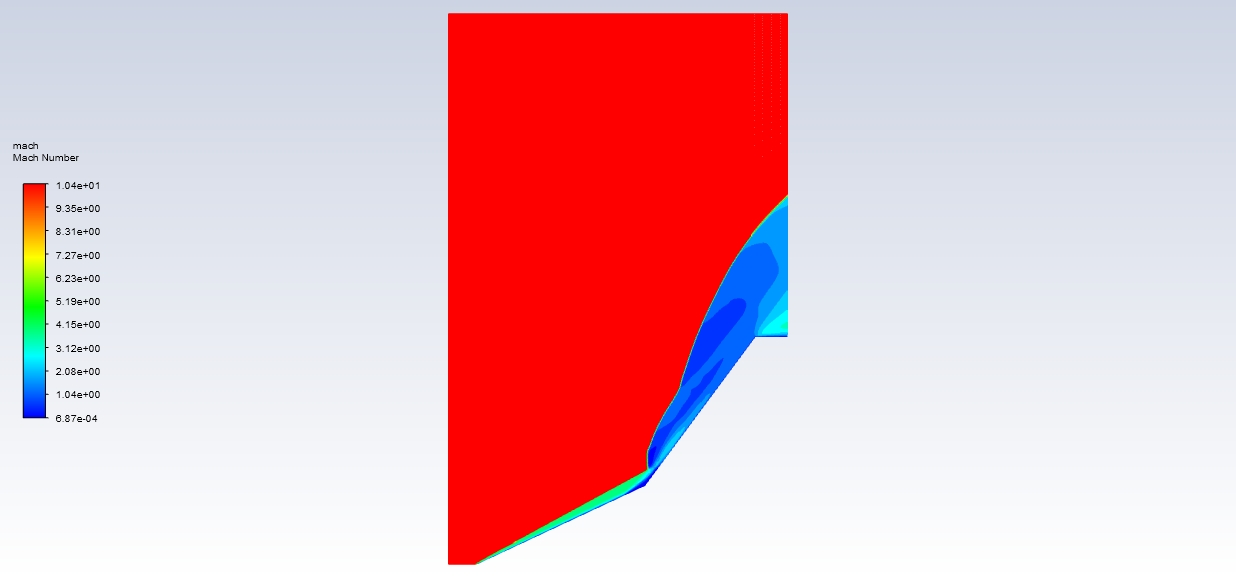
\includegraphics[width=0.7\linewidth]{images/mach_number_3663.jpeg}
  \caption{ Mach Number contour at 3.96 ms }
  \label{fig:mach_contour}
\end{figure}


\begin{figure}[ht]
\centering
  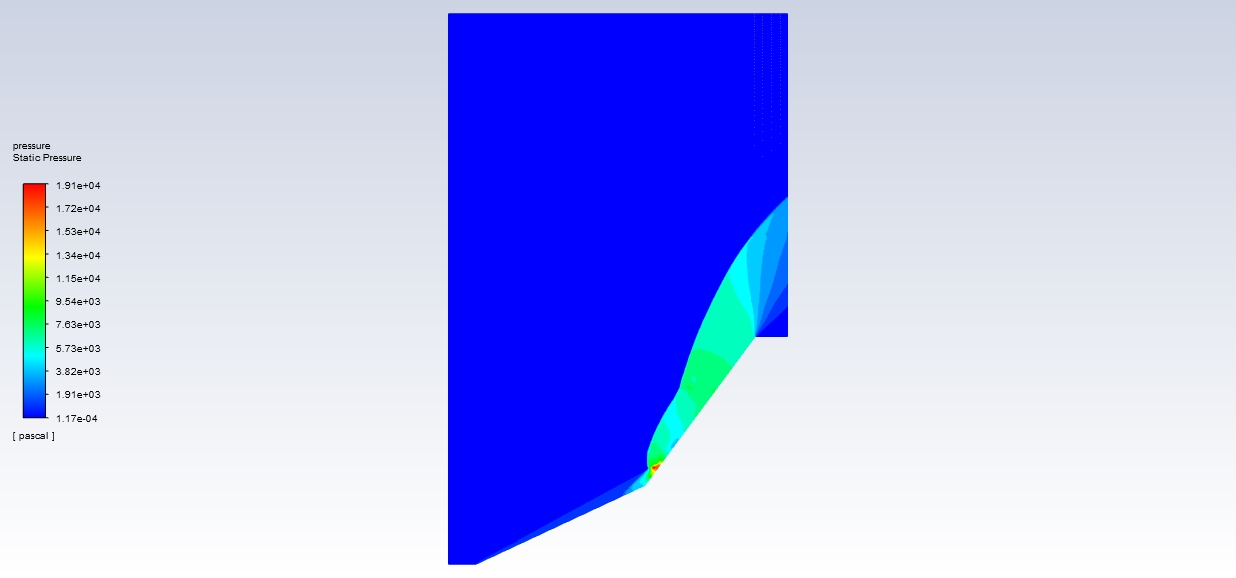
\includegraphics[width=0.7\linewidth]{images/pressure_contour_3669.jpeg}
  \caption{Pressure contour at 3.96 ms }
  \label{fig:pressure_contour}
\end{figure}
In Figure \ref{fig:mach_contour}, we can observe the formation of the bow shock in the aft wedge and the unsteadiness in the separation bubble. There is clear formation of triple and separation length can also be found to be varying. There is an expansion fan that is to be found the aft cone which tend to increase mach number thereby slightly increasing the temperature, After the shock interaction, that is the oblique shock hitting the boundary layer in aft cone, there is clear formation of shear layer near the aft cone and moving out of the cone geometry. After a few period of time, the reattachment of shock is found where the boundary layer shifts of from the aft cone and there is slip line formation in the flow process.

\begin{figure}[]
\centering
  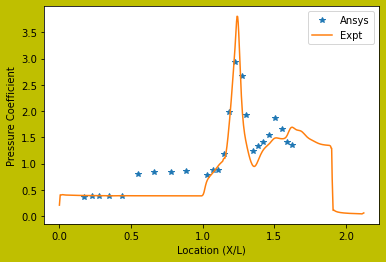
\includegraphics[width=0.6\linewidth]{images/PressureCoefficient.png}
  \caption{ Pressure Coefficient comparison from Experimental Data [7] to CFD Data }
  \label{fig:Cp}
\end{figure}


\begin{figure}[ht]
\centering
  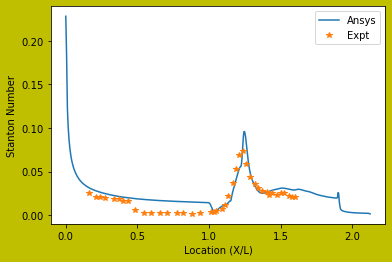
\includegraphics[width=0.6\linewidth]{images/Stanton Number.png}
  \caption{Stanton number comparison from Experimental Data [7] to CFD Data}
  \label{fig:Stanton_number}
\end{figure}

As observed in Figure \ref{fig:Cp}, the flow prediction around the wall is considerably accurate and has an error percentage of 50 \% in the forward wedge where the amount of heat transfer is very high and the temperature and pressure fluctuations are intense and requires a dense mesh around the region for the proper capturing of static and stagnation pressure. In the wedge or cross-section region where there is an inclination in the aft wedge, the pressure coefficient curve matches almost the same with respect to experimental data and has almost 16 \% difference in the peak stagnation pressure value. The main equation that is used to calculate the pressure coefficient is given in the equation below,

\[C_p = \frac{(P_0 - P_{\infty})}{(\frac{1}{2} \rho_{\infty} V_{\infty}^2)} \]

Stanton number which is the non dimensionalised number of heat transfer is shown in the Figure \ref{fig:Stanton_number}, the formula for Stanton number is given by 

\[St = \frac{Q_t}{( \rho_{\infty} V_{\infty}) (H_0 - H_W)}      [8] \] 

In the forward cone, the heat transfer prediction has an error of around 1\% and as it reaches the wedge centre the error continuously increases and reaches to 10 \% and there is an increase in the heat transfer in aft cone part since there is a sudden increase in heat transfer and the error is around 18 \% on the peak and later again reduces as the heat transfer reduces at the later stages of the wedge.